\chapter{Representation, Locality and Cost Argument}
\label{app:backend-argument}

This appendix gives the source-level argument used for the measured backend.
It makes the proof obligations readable independently of the repository's
review notes; the source correspondence is indexed in
\cref{app:claim-traceability}. It is a manual argument about the specified
operations, not a formal verification of Python execution. The geometric
precondition is a simple curve with distinct, totally ordered intersections.
The final cost statement uses unit-cost comparisons, machine-word operations
and constant-size allocation, with expected dictionary access and amortized
growth. Checked audits, replay and input certification are excluded.

\section{Decoding and Preservation}
\label{sec:proof-representation}

\begin{definition}[Complete representation $D$]
Decode each header as an ordered external red--black tree. External leaves
are black with rank zero and span one. An internal separator is the maximum
left key; its children have equal rank, and its rank is that common rank
plus one exactly when it is black. No red node has a red child, and the
complete root is black. Internal span means full leaf count in an interior
node, inward-branch count on a rib, and zero at the root. Header size is the
total leaf count, including for a singleton.

On a left rib the left slot points up; on a right rib the right slot points
up. The other slot points inward. Decoding reverses these outer chains;
off-rib children already point down. Internal-root slots are empty, and
header top caches identify its two logical children. Fingers identify extreme
leaves; decoding is acyclic and reaches every node once. Stable leaf/handle
identities bind pair records. Only endpoints carry boundary-header references.
Each live header has one owner and occurs in that owner's ordered slots,
of which there are at most two.
\end{definition}

\begin{figure}[!htbp]
 \centering
 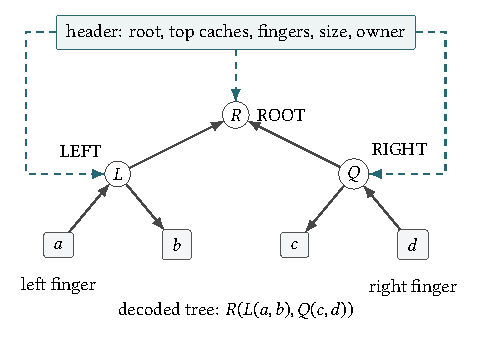
\includegraphics[width=.72\textwidth]{heterogeneous_representation.pdf}
 \caption{Physical decoding: solid arrows are node links; dashed arrows are
 header references. Outer chains point up and inward branches down; root
 slots are empty. Header fingers reference leaves $a,d$ (arrows omitted).
 Colours and sizes are omitted.}
 \label{fig:proof-representation}
\end{figure}

\begin{lemma}[Conversion and endpoint insertion]
\label{lem:proof-insert}
Conversion between a downward component and its finger representation
preserves its decoded leaf sequence and identities. Singleton creation and
legal endpoint insertion restore $D$ without scanning inward subtrees.
\end{lemma}
\begin{proof}
When exposing a rib, save its outward child before replacing that slot by
the upward link. The processed chain and untouched remainder still decode
to the original tree; each new rib span is the unchanged inward count.
The inverse saves the upward link, attaches the already processed lower
component and refreshes rank and full span bottom-up. A leaf needs no
conversion; a nonroot top exposes one rib, an internal root two. Final root
blackening may increase rank by one.

Insertion attaches a black leaf and red connector at the selected finger.
Only the connector's upper edge can violate red adjacency. A red uncle is
blackened with the parent while the grandparent becomes red; the latter's
rank is unchanged and the conflict moves upward. With a black uncle the
left-side rotation is
$G(P(C,M),F)\mapsto P(C,G(M,F))$.
Initially $P,C$ are red and $G,F$ black. The three blocks $C,M,F$ have equal
rank. Afterwards $G$ is red, $P$ black, and the total rank is unchanged.
Separators remain $\max M$ at $G$ and $\max C$ at $P$.

For nonroot $G$, it becomes interior with children $M,F$; $P$ retains its
rib role, points to the former ancestor and has inward child $G$. For root
$G$, $P$ becomes the empty-slot root, $G$ becomes the opposite rib with
inward child $M$, and top caches become $C,G$. The unchanged upward links
from $C$ and $F$ already name their correct parents. Spans follow these roles.
The mirror is $G(F,P(M,C))\mapsto P(G(F,M),C)$, with separators $\max F$
and $\max M$, still maxima of left blocks. Black-parent termination,
rotation or root blackening restores $D$. Only the replaced endpoint's
boundary slot changes; the live list ID is retained.
\end{proof}

\begin{lemma}[Recursive downward join contract]
\label{lem:proof-join}
Joining two disjoint ordered components preserves their leaf union and order.
The recursive return has equal child black heights and correct metadata, but
may contain one root--child red edge when its root is red. A complete
nonempty join restores the red--black invariants.
\end{lemma}
\begin{proof}
Both input roots are blackened before descending the taller component's
inner path. At equal-rank black roots, a red connector forms an internally
valid base case with the same rank. On return, the replaced component keeps
that rank. A black parent with no conflict is refreshed. For LL, LR, RR or RL
conflicts, one or two rotations create a red middle root with two black
children and unchanged black height. Thus the returned subtree is internally
valid, although its root can conflict with the caller.

A red parent takes the direct-return branch. Its originally black updated
child can return an internally valid red root; the other child stays black.
Consequently only the updated root--child edge may be red--red. This is a
recursive transient, not $D$. The original parent of that red node is black
and repairs precisely this LL/LR/RR/RL conflict on the next return. The
induction excludes a deeper or second simultaneous red conflict. Descent
never searches through a return transient.

At the top, either the valid base case or a black-root repair returns an
internally valid tree. Final root blackening changes only root colour; it
cannot repair an internal red edge. For example, joining
$A_B([0],P_R([1],[2]))$ to $[3]$ temporarily returns
$P_R([1],C_R([2],[3]))$, then repairs at $A_B$; the mirror uses LL.
In a left rotation $A(X,B(Y,Z))\mapsto B(A(X,Y),Z)$, separators stay
$\max X,\max Y$; refreshing bottom-up gives full spans and ranks.
The connector separator is the left input's maximum and sizes add.
An empty-input branch simply returns the other component and retires the
unused connector; this branch alone need not blacken its root.
\end{proof}

\begin{lemma}[Detachment and split preservation]
\label{lem:proof-split}
Legal split and adoption preserve the leaf set, stable identities and
descendant groups, and restore $D$ and header ownership at their completion.
\end{lemma}
\begin{proof}
Detachment removes an extreme component and its parent connector, replacing
the latter by its sibling. A red parent loses no black height; a red sibling
replacing a black parent is blackened. Otherwise the replacement is short by
one black layer. Use a transient $D^*$: the short component's rank is actual,
but ancestors still account for one virtual black layer on that path.
Refreshing these ancestors as ordinary equal-height trees would be invalid.

For short rank $r$, the sibling has rank $r+1$, so is not a leaf.
A red sibling is blackened and the black parent reddened before rotation,
reducing to a black sibling. If both nephews are black, redden the sibling:
a red parent absorbs the deficit by blackening; a black parent decreases
rank and becomes the next short component. A red near nephew with black far
nephew is rotated and recoloured into the far-red case. In that case the
sibling takes the parent colour, the parent and far nephew become black,
and a rotation absorbs the deficit. A deficit reaching the root lowers the
whole black height by one. These are all repair branches.

For a left deficit the outer rotation is
$P(S,B(N,F))\mapsto B(P(S,N),F)$, with separators $\max S,\max N$.
$P$ is a left rib pointing up to $B$ and inward to $N$, with span $|N|$.
At the root, $B$ gets empty slots, span zero and top caches $P,F$;
otherwise it retains the rib with inward $F$ and the old upward link.
The mirror keeps separators $\max F,\max N$ in
$P(B(F,N),S)\mapsto B(F,P(N,S))$.
A near rotation at the opposite root rib changes
$B(N(X,Y),F)$ to $N(X,B(Y,F))$: the inward spans become $|X|,|Y|$,
and the appropriate top cache becomes $N$. The far upward link is unchanged.
These substitutions preserve order and update only affected metadata.

The selected component need not straddle the cut: it can lie wholly on one
side. The remainder lies wholly on a known output side. Downward splitting
classifies leaves by key $\leq v$ or $>v$; each saved sibling is joined once
to the corresponding accumulator in order, using \cref{lem:proof-join}.
Connectors are reused once or retired, never leaves. Finger joins stop at
equal black rank and use \cref{lem:proof-insert}; conversion handles their
component boundaries. Size starts at one at a finger and accumulates inward
spans on ascent; at the root use header size. The remainder is obtained by
subtraction, downward sizes by full spans, and joined sizes by addition.
There is no output-wide counting pass.

Every split retires the source header, including an empty-side fast return,
and allocates fresh IDs for nonempty outputs. It clears old endpoint
references and sets new ones. Adoption checks the pending source, owner,
new parent and output IDs, then changes headers and at most two child slots.
Leaves, handles and their own child groups are unchanged. Strict containment
of extreme children implies containment of the whole ordered group. In the
sorting call the new parent was childless, so acquiring its strictly contained
old children cannot create a cycle. Pending overlap is allowed only for this
planned transfer; completion clears it before output insertion.
\end{proof}

\begin{figure}[!htbp]
 \centering
 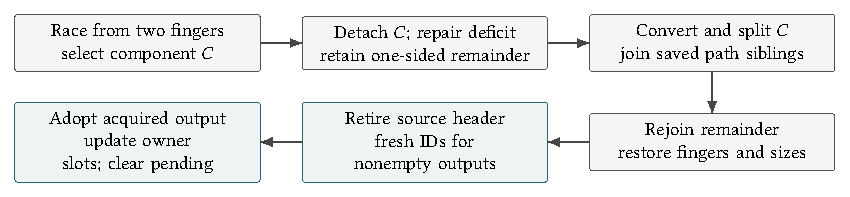
\includegraphics[width=\textwidth]{heterogeneous_split_flow.pdf}
 \caption{Two-sided split and adoption. The selected component may itself
 yield an empty side. Sizes come from path spans and header totals; transfer
 changes header ownership rather than rebinding every leaf.}
 \label{fig:proof-split-flow}
\end{figure}

\section{Locality and Exact Grouping}
\label{sec:proof-locality}

Use $G$ from \cref{sec:algorithm-sibling-lists}, not merely a bound of two
groups. An owner is the smallest strictly enclosing same-parity pair, or
the parity dummy. Its region $R$ is bounded by its arc and its direct
children's arcs, with intervening open axis gaps. Descendant arcs lie
behind child boundaries, not inside $R$.

\begin{lemma}[Applicable re-entry gaps]
\label{lem:proof-reentry}
Suppose the region has not changed since its latest member $P_j$ was added.
If $P_j$ is a child, first re-entry from $z_j$ uses its adjacent region gap,
or, for the dummy, the opposite unbounded gap. In the latter case, $z_j$
and the re-entry point $z_k$ bracket all other finite endpoints of the
region. If $P_j$ is the finite parent, first re-entry uses the gap
immediately inward from $z_j$.
\end{lemma}
\begin{proof}
The child case is the locality lemma of
\textcite[p.~88, locality lemma (a)--(b), Figs.~3--4]{fung1990simplified},
under its latest-child and unchanged-region hypotheses; part (b) supplies
the dummy bracketing condition. It is not applied to a latest finite parent.
For that additional case let $q$ be the first child endpoint inward from
$z_j$, or the other parent endpoint if there is no child.

Assume the first re-entry $z_k$ is outside $(z_j,q)$. Choose a child endpoint
$a$ strictly between $z_j$ and $z_k$ along that boundary, and let
$b=z_{j-1}$ be the other parent endpoint. An auxiliary simple crosscut
inside $R$ connects $z_j$ to $z_k$ and separates these boundary vertices.
The actual curve portion from $z_j$ to $z_k$ lies outside $R$ by first
re-entry and meets the crosscut only at its ends. Together they form a simple
closed curve separating $a$ and $b$. The old curve portion connecting $a$
to $b$ cannot cross the crosscut, because the old curve avoids the region's
interior; it cannot meet its newer endpoints or cross the actual later
portion, by simplicity. This contradicts separation. If there is no child,
the entire inward gap is already $(z_j,q)$. Unlike the dummy, a finite parent
has no second unbounded outside gap. This establishes the extra case.
\end{proof}

\begin{lemma}[Legal calls and prefix induction]
\label{lem:proof-locality}
Starting from initialization, $G$, geometric ownership and the sorted-prefix
invariant imply legal endpoint insertion, same-owner/different-group transfer
when required, and correct output insertion. Each completed iteration restores
these invariants.
\end{lemma}
\begin{proof}
Initialization has one singleton per parity family and correctly orders three
points. Consider iteration $i$, with $x=z_{i-1}$ and new point $y=z_i$.
Let $p$ be the smallest same-parity interval containing $x$, or the dummy,
and let $P_j$ be the latest member of its owner region. Updates inside older
descendants have not changed that region. Were there an earlier first
re-entry, its next same-parity arc would create a new direct child of $p$,
possibly acquiring consecutive children. Its end index would exceed $j$,
contradicting the definition of $j$. Here alternation between the two
parities is essential. Thus \cref{lem:proof-reentry} applies to $x$.

Except for $x$ and, at odd $i$, $z_1$, processed points are endpoints of
same-parity pairs. Step~1/2 skips this exceptional $z_1$. Parent and direct
child endpoints block all more distant ancestors and descendants in the
neighbor search. Consequently an interior entry gap gives the last endpoint
of the left group and first endpoint of the right group; an outer gap gives
one group boundary and the parent. By $G$ these are designated endpoints,
not arbitrary members. The two groups, when both present, have the same owner
and different live IDs.

For $x<y$, simplicity implies that $y$ remains inside finite $p$ and is
neither inside a direct child's interval nor equal to its endpoints.
If the left boundary is $p$, Step~3(a) creates a singleton in a free slot.
In the dummy outer-gap case, the bracketing condition leaves the group
beyond $z_j$ empty, so the owner has at most one group. When the left
boundary is a child, Step~3(a) instead appends to the left group. If the right boundary is $p$,
there are no children to transfer. Otherwise its right group is the source.
Reading that source before insertion is safe: Step~3(a) changes only the
other group or a new slot, preserving source identity and owner.

All source children lie to the right of $x$. Since $y$ cannot lie inside a
child, a source key $\ell_h\leq y$ is equivalent to
$x<\ell_h<r_h<y$. Hence value splitting acquires precisely the consecutive
children enclosed by the new pair. The temporary overlap is exactly the
declared transfer. After adoption, $p$'s latest child is $P_i$ and its groups
are separated by $y$; $P_i$ is the latest parent of its own single acquired
group. Other owners' groups, descendant identities and the opposite parity
are unchanged. Strict enclosure gives acyclicity.

Among old paired endpoints between $x$ and $y$, the largest is the high
endpoint of the rightmost acquired direct child, or $x$ if none exists.
Descendants cannot exceed that child's extreme. This is the predecessor
ignoring the exceptional odd-stage $z_1$; replacing the anchor by $z_1$
exactly when it lies between this base and $y$ gives the true predecessor.
The decreasing case reflects the argument, using the low endpoint and
successor. Step~3(c) therefore preserves sorted order after the pending-state
fence. This proves the simultaneous prefix induction.
\end{proof}

\section{Costs of Mixed Operations}
\label{sec:proof-cost}

\begin{lemma}[Cumulative join cost]
\label{lem:proof-telescoping}
Splitting a downward component of raw rank $r$ costs $O(r+1)$ in joins and
path work. It does not require $O(r)$ joins each independently charged $O(r)$.
\end{lemma}
\begin{proof}
Write $\nu$ for rank after blackening the root. For nonempty join inputs of
normalized heights $a,b$, the result has height $c$ and descent count $Q$ with
\[
 \max(a,b)\leq c\leq\max(a,b)+1,\qquad Q\leq2|a-b|+3.
\]
Descent follows a legal tree: each black level decreases the height difference
and there cannot be consecutive red nodes. Each return repair is constant
work by \cref{lem:proof-join}. An increase in height leaves a black root with
black children: before final blackening it was the valid red base or a
black-root repair result, not the red-root transient. Pre-blackening an
originally red input adds at most one separately.

Inductively, splitting a legal raw-rank-$r$ component gives nonempty outputs
of normalized height at most $r+1$. For a black input attaining $r+1$,
the output root and children are black. For the induction step let child
rank be $q$. At a black root, both join inputs have normalized height at
most $q+1$, so the output is at most $q+2=r+1$, with the stated strong case.
At a red root the children are black. If the recursive output reaches
$q+1$, its root and children are black by that strong case; joining a
height-$q$ sibling descends one level and cannot increase height again.
Otherwise the ordinary join bound suffices.

Thus at each backtracking join, accumulated height $a$ and untouched sibling
height $b$ satisfy $a-b\leq1$. The displayed bounds imply
$Q\leq2(c-a)+5$. Each of the two output accumulators has nondecreasing
normalized height, bounded by $r+1$. Summing over $J=O(r+1)$ joins gives
$\sum Q\leq2(\nu_L+\nu_R)+5J=O(r+1)$. Empty-side returns add only constant
work per frame. This pays descent, reconstruction and metadata maintenance.
\end{proof}

\begin{lemma}[Finger distance and opposite-rib work]
\label{lem:proof-finger}
For smaller nonempty output size $s$, the selected component has rank
$r=O(\log(s+1))$. Opposite-rib access in detachment costs $O(r+D+1)$,
where $D$ counts continuing deletion propagations.
\end{lemma}
\begin{proof}
The left search climbs only while the parent separator is below the cut;
the right search has the reflected condition. It is the component
\emph{before} a climb that is known to be wholly on one side, not necessarily
its parent. A one-sided component of rank $t$ has at least $2^t$ leaves.
On the smaller side this is at most $s$, and one climb increases rank by
at most one. Alternating searches differ by at most one step; no two red
levels are consecutive. Hence both paths, and the selected component,
have the stated rank bound. If $s=0$, the endpoint fast path costs $O(1)$.

An inward sibling is interior except at the root. Only there can
\texttt{rib\_child} require an opposite-rib walk. A red-sibling root rotation
makes the continuing parent nonroot; propagation at the root terminates.
A near rotation permits at most one additional far-nephew lookup.
There are therefore at most two such walks per repair. With initial short
rank $r_0\leq r+O(1)$, each continuing propagation raises actual rank by one;
the reached root has rank at most $r_0+D+2$.
This proves the walk bound. Conversion visits $O(r+1)$ levels;
finger joining climbs the large component only to the small component's
rank, also $O(r+1)$. Any ensuing insertion propagation is charged next.
\end{proof}

\begin{lemma}[One potential across mixed updates]
\label{lem:proof-mixed}
Endpoint insertion costs amortized $O(1)$, and split costs
$O(\log(s+2))$, including local repairs, conversion and size maintenance.
Creation and adoption have constant cost.
\end{lemma}
\begin{proof}
On decoded logical internal nodes define
\[
 \Phi=\#\{\text{black nodes with two black children}\}
       +2\#\{\text{black nodes with two red children}\}.
\]
Count each node once across the live forest and temporarily disjoint
components; never reset the potential when headers change. Leaves contribute
zero. An insertion propagation changes a black/red-red grandparent of
weight two into a red node of weight zero; the blackened parent is mixed
and the blackened uncle has two black children, contributing one.
The decrease is one per continuing propagation. An upper boundary or terminal
repair changes only constantly many weights.

In a continuing deletion propagation, the black sibling with black children
becomes red, losing one, and the black parent changes from two black children
to mixed, losing another. The next ancestor's child stays black. Thus each
such step decreases $\Phi$ by two; absorption, rotations and root treatment
change constantly many weights. Direction conversion alone changes neither
logical children nor colours. The $O(r+1)$ join/path steps each affect a
constant number of weights, and any finger-join propagation uses this same
potential. For constants independent of the sequence,
\[
 \Delta\Phi\leq C(r+1)-D-I,\qquad
 W\leq C'(r+D+I+1),
\]
where $I$ counts propagation rounds, not individual recolourings.
Choose a sufficiently large constant multiplier of $\Phi$ to pay both
propagation and the $D$ term in the opposite-rib work.
\Cref{lem:proof-telescoping,lem:proof-finger} then give the split bound.
The same accounting with constant boundary work gives endpoint insertion.
Adoption touches bounded header/owner slots, not a leafwise ownership map.
\end{proof}

\begin{theorem}[Total valid-input work]
\label{thm:proof-total}
Under the stated computation model, the shared minimal core with this
finger backend uses $O(n)$ expected/amortized work and $O(n)$ space on
a valid input of length $n$.
\end{theorem}
\begin{proof}
By \cref{lem:proof-locality}, each iteration performs constantly many legal
boundary accesses and at most one creation/insertion, split and adoption.
To pay the split terms use the nonnegative list potential
$\Psi=c\sum_{L\ne\varnothing}(|L|-\log_2|L|)$.
Creation increases it by $c$; insertion into size $m$ increases it by
$c(1-\log_2(1+1/m))\leq c$; adoption changes no sizes. For a nonempty
split $m=a+b$ with $1\leq a\leq b$,
\[
 \Delta\Psi=c\log_2\frac{a+b}{ab}
       \leq c(1-\log_2 a).
\]
Since $\log_2(a+2)\leq\log_2a+\log_2 3$, a sufficiently large $c$
pays the smaller-side term. An empty-side split has $\Delta\Psi=0$ and
constant amortized cost. Combine this with the single multiple of $\Phi$
in \cref{lem:proof-mixed}; initialization has constant potential.

The remaining shared-core work consists of bounded endpoint/handle and
owner-slot accesses, geometric comparisons, stage records and linked output
insertion per iteration. It performs no membership or ancestor scan in this
backend. Input materialization and final output traversal are linear.
Access wrappers and iterator resumption add constant work per affected access,
not zero work. Constant-size records per iteration and linear node/handle
registries give the space bound, including retired-header bookkeeping.
Nonnegative final potentials complete the aggregate bound.
\end{proof}

This theorem concerns source-level work in the specified model. It neither
charges complete audits and replay to the sorter nor predicts Python wall
time, an uninstrumented implementation, or a practical crossover.
